Før vi har låst os fast på et bestemt design, har vi søgt inspiration andre steder. Vi fandt det interessant at undersøge hvordan forskellige netbankers layout så ud, da de i bund og grund har med samme problemstilling at gøre. De forskellige netbanker har hver især meget forskellige tilgange til layoutet, nogle er meget simple og overskuelige, andre er mere komplicerede og kan nogle flere ting. Vi vil i dette afsnit kigge på de bankers layout, vi har fundet inspirerende, og på et enkelt eksempel vi ikke har fundet brugbart.

Danske Bank har siden slutningen af 2012 løbende lanceret et nyt layout til deres netbank\cite{Danskebank}. Dette skulle give kunderne et langt bedre overblik over hvad deres penge er gået til, og hvor meget de bruger i forhold til hvad de tjener. Generelt set giver det nye layout kunden et langt bedre overblik over deres økonomi. Det nye design er bygget op, således at samtlige udgifter er blevet kategoriseret. Kategorierne kan f.eks. være bolig, dagligvare eller øvrige. Ydermere kan kunden vælge en kategori og dermed få en liste over alle de udgifter, der har været under denne kategori. 

\begin{figure}[h!]
\centering
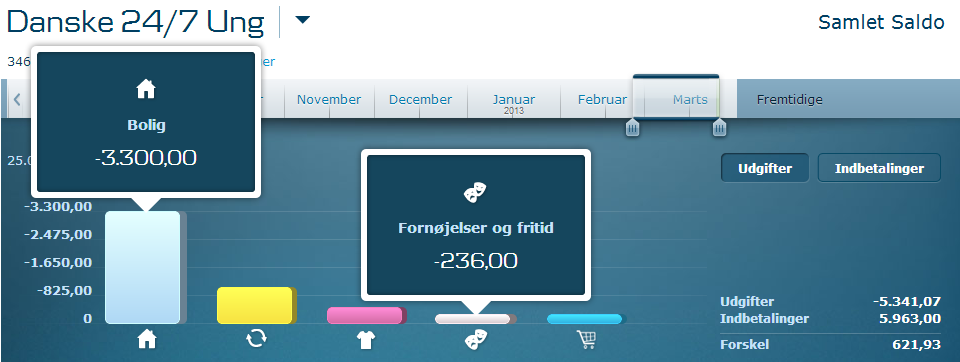
\includegraphics[width=1.0\textwidth]{Billeder/DanskeB.png}
\caption{ Illustrationen viser kategoriseringen af kundens udgifter.}
\label{DanskeB}
\end{figure}

Vi ser på \ref{DanskeB} at man ud fra denne lille del af ens kontooversigt, har mulighed for at se kontoens samlede saldo, forskellen på indtægter, udgifter og hvad pengene er gået til. Kategoriseringen, det vil sige alle søjlerne, er sorteret efter største beløb, denne sortering kan ændres til dato eller tekst. Den sidste detalje vi vil nævne om billedet er, at man har mulighed for at ændre tidsintervallet, så man kan kontrollere lige præcis den periode man ønsker. Yderligere er der, lige under \ref{DanskeB}, en oversigt over alle udgifter og indtægter. Se evt. [[Bilag xx]]

Spar Nord har haft en lidt anderledes tilgang til samme problemstilling. I Danske Banks udgave møder du diagrammet som det første når du åbner en konto, hvorimod du hos Spar Nord møder den klassiske oversigt over kontobevægelser. Den klassiske oversigt dækker om en datosorteret liste over udgifter og indtægter. Se evt. figur \ref{BasisB}. Herefter kan du vælge at få en oversigt over dit forbrug udformet i et cirkeldiagram. En anden forskel er måden du vælger tidsinterval på, hos Danske Bank “rykker” du interaktive pile til det ønskede tidspunkt og interval, hos Spar Nord får du forskellige muligheder, såsom “seneste 30 dage” eller én bestemt måned. \ref{SparN} Dette vil sige at Danske Banks interval-mulighed er mere fleksibel.

\begin{figure}[h!]
\centering
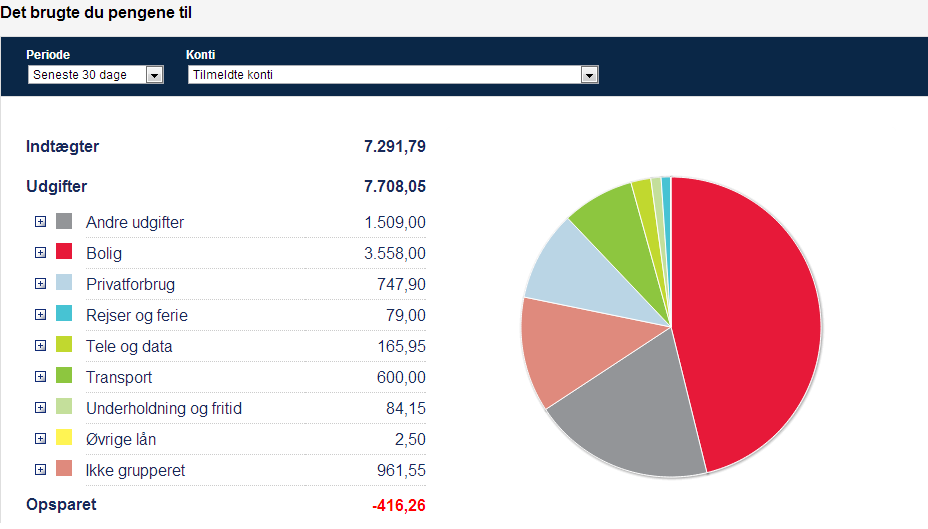
\includegraphics[width=1.0\textwidth]{Billeder/SparN.png}
\caption{ Billedet viser hvordan Spar Nord har valgt at visualisere kontooversigten.}
\label{SparN}
\end{figure}

Udover de førnævnte forskelle er de to modeller i bund og grund ens. Det er dog langt fra alle banker, der tilbyder kunderne et visuelt overblik. Flere banker lister udelukkende indkomst og forbrug i kronologisk rækkefølge, en model blandt andet Danske Bank også havde før i tiden. Et eksempel herpå er Basisbank, de har netop valgt et simplificeret layout. Se figur\ref{BasisB}. Dette 

\begin{figure}[h!]
\centering
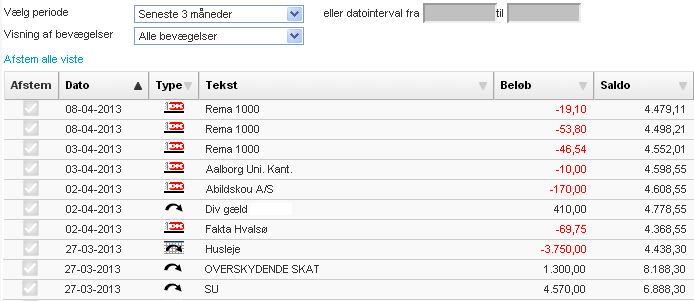
\includegraphics[width=1.0\textwidth]{Billeder/Basisbank.png}
\caption{ Illustrationen viser hvordan en konto hos BasisBank kan se ud.}
\label{BasisB}
\end{figure}

Spørgsmålet er så hvad vi kan bruge al denne viden til. Én ting er sikker, hvis vi vælger at anvende noget lignende disse modeller, så bliver det på en omvendt måde. Omvendt skal forstås således at vi, i vores program, ikke har tænkt os at liste udgifter, derimod indtægter børnene får. Dette vil være mere relevant for børnene da de ikke har et betalings-/hævekort tilknyttet deres konto, og dermed ikke selv kan hæve penge fra kontoen. Hvis vi tager udgangspunkt i, at vi vælger en model der ligger tæt op ad disse to gennemgåede modeller, kan kategorierne kan i stedet for bolig, dagligvarer og øvrige, være opvask, støvsugning og øvrige. På denne måde kan barnet danne sig et overblik over hvilke pligter der er tjent flest penge på. Man kunne også implementere andre kategorier, kategorier der har med økonomiske aspekter at gøre. Således at barnet kan se i hvilken betydning fx rente har for det samlede beløb. En anden ting man kunne hente direkte fra netbankerne, er forskellen mellem indtægt og forbrug, og naturligvis vil det være oplagt at have den samlede saldo ret synlig. 

Hvorvidt vi vælger at bruge et cirkeldiagram kontra et søjlediagram, eller måske noget helt tredje, og andre ting såsom om tidsintervallet er vigtigt for vores program, vil senere blive afgrænset i [[ref afsnit design afgrænsning]].






%[[Bilag xx]]












%[[Bilag xy]]
%Eksisterer ikke endnu!!
